
\documentclass[journal]{IEEEtran}
%\usepackage{mathtools}
\usepackage{graphicx}
\usepackage[font=footnotesize,labelfont=bf]{caption}
\usepackage{subcaption}
%\usepackage{xcolor,colortbl}
\usepackage{amsmath}
\usepackage{amssymb}
\usepackage{float}
\usepackage[table,xcdraw]{xcolor}
\usepackage{latexsym}
\usepackage{wrapfig}
\usepackage{etoolbox}
\usepackage[doublespacing]{setspace}


\ifCLASSINFOpdf
  % \usepackage[pdftex]{graphicx}
  % declare the path(s) where your graphic files are
  % \graphicspath{{../pdf/}{../jpeg/}}
  % and their extensions so you won't have to specify these with
  % every instance of \includegraphics
  % \DeclareGraphicsExtensions{.pdf,.jpeg,.png}
\else
  % or other class option (dvipsone, dvipdf, if not using dvips). graphicx
  % will default to the driver specified in the system graphics.cfg if no
  % driver is specified.
  % \usepackage[dvips]{graphicx}
  % declare the path(s) where your graphic files are
  % \graphicspath{{../eps/}}
  % and their extensions so you won't have to specify these with
  % every instance of \includegraphics
  % \DeclareGraphicsExtensions{.eps}
\fi

\usepackage{graphicx}
\usepackage{amssymb,amsmath,bm,balance	}
\usepackage{textcomp}


\hyphenation{Audio Speech and Language Processing}


\begin{document}

\title{Robust Speaker Recognition in Co-channel Speech \\
		Using Probabilistic Linear Discriminant Analysis}
%
%
% author names and IEEE memberships
% note positions of commas and nonbreaking spaces ( ~ ) LaTeX will not break
% a structure at a ~ so this keeps an author's name from being broken across
% two lines.
% use \thanks{} to gain access to the first footnote area
% a separate \thanks must be used for each paragraph as LaTeX2e's \thanks
% was not built to handle multiple paragraphs
%

\author{Navid~Shokouhi,~\IEEEmembership{Student Member,~IEEE,}
	John~H.~L.~Hansen,~\IEEEmembership{Fellow,~IEEE}}

\maketitle


%\begin{abstract}
%The abstract goes here.
%\end{abstract}

% Note that keywords are not normally used for peerreview papers.
\begin{IEEEkeywords}
Co-channel speech, speaker recognition, probabilistic linear discriminant analysis
\end{IEEEkeywords}






% For peer review papers, you can put extra information on the cover
% page as needed:
% \ifCLASSOPTIONpeerreview
% \begin{center} \bfseries EDICS Category: 3-BBND \end{center}
% \fi
%
% For peerreview papers, this IEEEtran command inserts a page break and
% creates the second title. It will be ignored for other modes.
\IEEEpeerreviewmaketitle



\section{Introduction}
\label{sec:introduction}


\begin{figure}[b]
	\hrule
	\vspace{.03cm}
	{\rmfamily{\small \em { Mail All Correspondence To:}\vspace{-0.2cm}\\}}
	\begin{minipage}{0.2\linewidth}
		\centering
		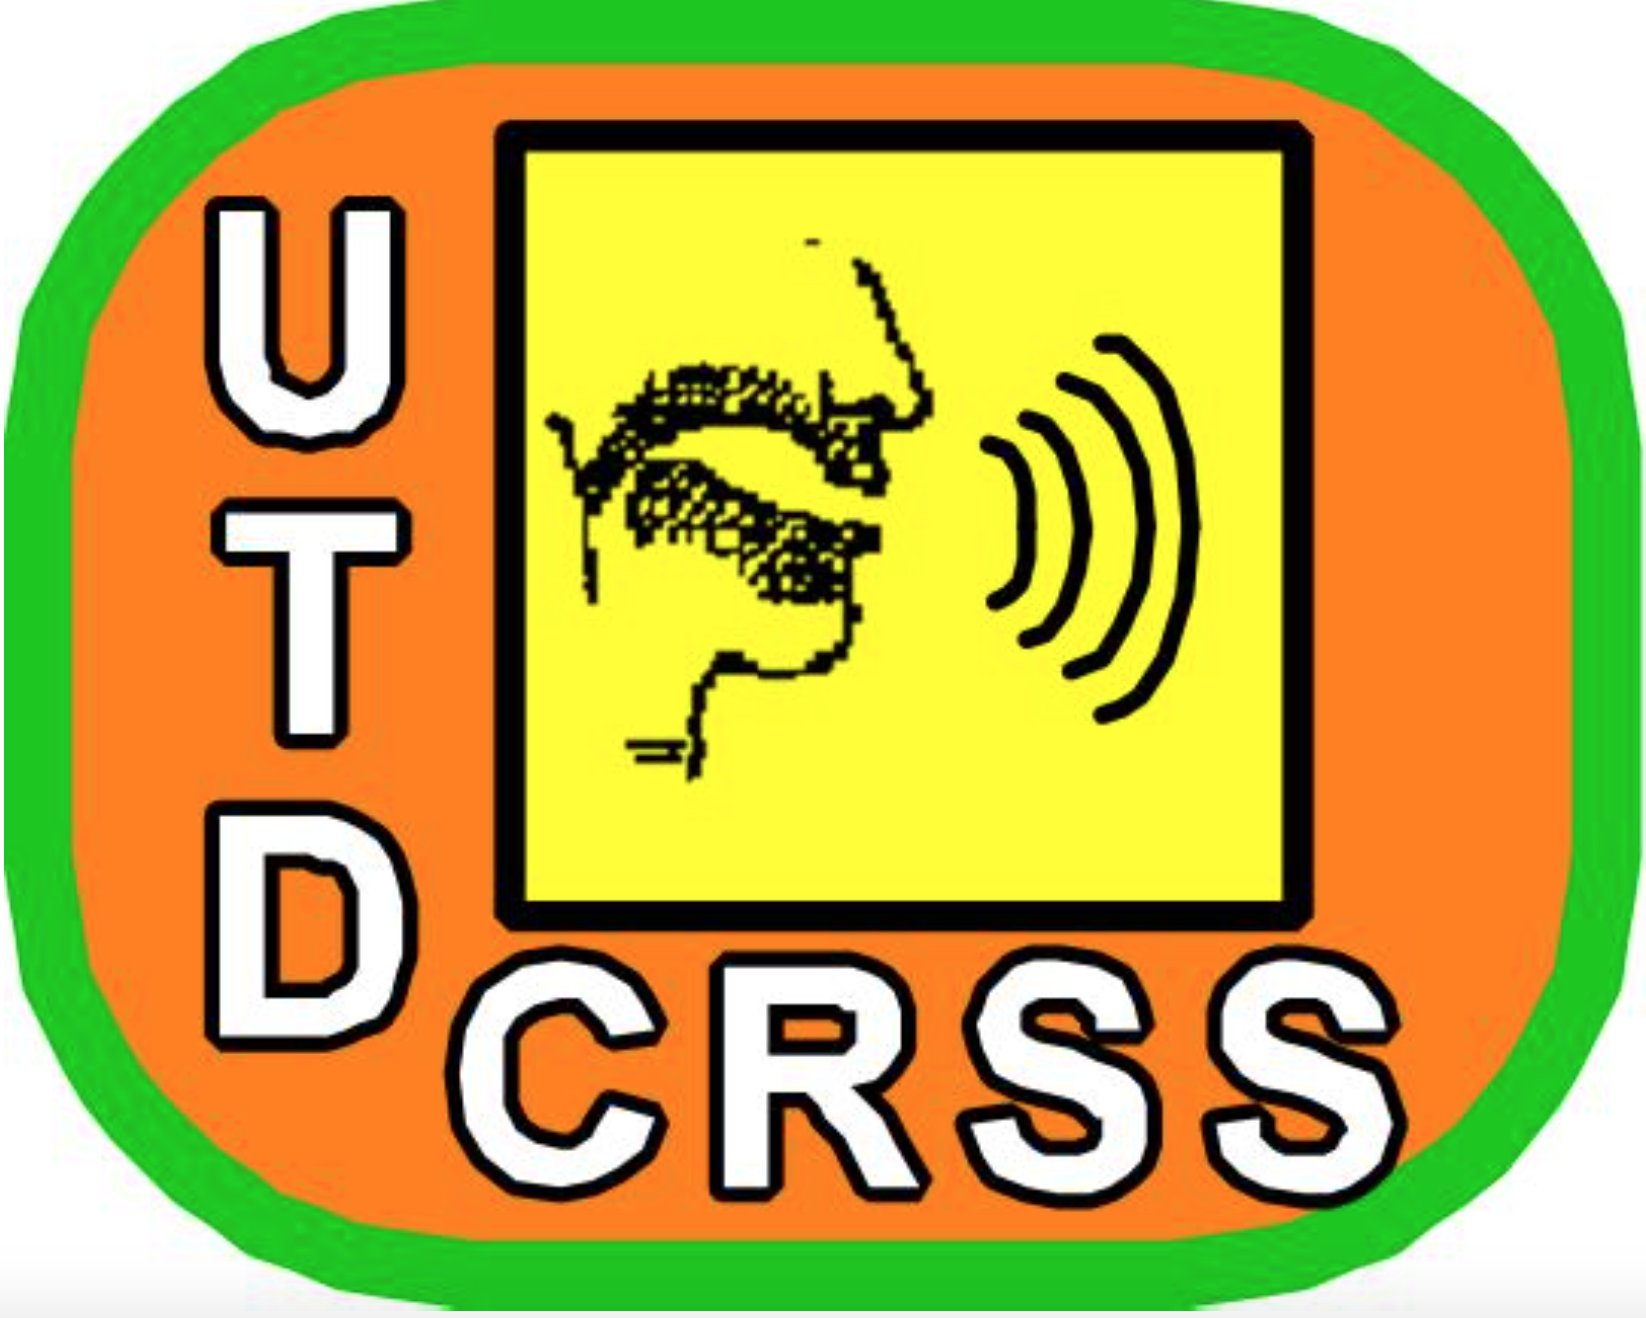
\includegraphics[width=1\linewidth]{figures/CRSS_logo}
	\end{minipage}
	\begin{minipage}{0.8\linewidth}
		\begin{singlespace}
			\small \vspace{.5cm}
			\footnotesize
			Prof. John H.L. Hansen\\
			Center for Robust Speech Systems (CRSS), Erik Jonsson School of Engineering and Computer Science, Dept. of
			Electrical Engineering, University of Texas at Dallas\\
			2601 N. Floyd Road, EC33, Richardson, TX 75080-1407, U.S.A\\
		\end{singlespace}
	\end{minipage}
	\small{$^*$This project was funded by AFRL under contract FA8750-12-1-0188 and partially by the University of Texas at Dallas from the Distinguished University Chair in Telecommunications Engineering held by J.H.L. Hansen.}\\
\end{figure}


\IEEEPARstart{C}o-channel speech refers to single-channel audio signals that contain more than one speaker. 
In this study, we address the problem of speaker recognition for co-channel recordings.
Co-channel speech refers to single-channel audio signals that contain more than one speaker. 
The presence of speech interference is an important artifact for all automatic speech processing systems. 
As speech technology continues to advance, the need to address multi-speaker interference increases. 

The difference between what we present here and every other study in this area is that we would like to bypass solutions that require removing interfering speech from the original signal, which are primarily known as speaker diarization. Speaker diarization is defined as the task of determining ``who spoke when?'' within an audio recording. 
Speaker recognition in co-channel speech using diarization as a preprocessing step involves recognizing each speaker within the recording, which is itself a speaker recognition problem. 
One can easily see the inherent logical issue in this approach; where in order to achieve $\bf A$, $\bf B$ is required. And performing $\bf B$ requires some variation of $\bf A$.
Alternatively, we are interested in modifying model parameters extracted from co-channel data in a way that would only represent the primary speaker. 
Currently, the most common parameterization of speaker dependent models is in the form of i-vectors~\cite{dehak2011front}. 
I-vectors are latent parameters that model the covariance of speaker/session-dependent Gaussian mixture models (GMM) with respect to a generic GMM (aka Universal background model). The UBM is ideally both session- and speaker-independent.
The use of i-vectors, has become a standard way of modeling speaker specific traits for speaker recognition. 
In a way that in many cases i-vector extraction is considered a preprocessing step in performing speaker recognition on a data-set. 
Therefore, it is both reasonable and desirable to concentrate on post i-vector analysis to deal with co-channel speech interference~\cite{ivector_challenge}. 
The goal of this study is to build upon the latent variable perspective, popularized by i-vectors~\cite{dehak2011front} and its predecessors~\cite{kenny2014jfa}, to improve speaker recognition in co-channel signals. 
This provides the luxury of short-circuiting speaker diarization, which in addition to what we described above is also a computationally intensive solution. 

Speaker recognition experiments can be highly influenced by the presence of secondary speakers, due to reduced reliability of the trained models. 
Although the target speaker is a common factor in all training samples for a given speaker model, the standard structure of speaker recognition systems has not been designed to average out interfering speech. 
To the best of our knowledge, there are few studies that address speaker recognition in co-channel speech signals. 
In~\cite{yantorno_report,yantorno_SID}, a description of the effects of artificially adding overlapped speech to train and test data in a Gaussian mixture model (GMM) based system is presented. 
There, the approach was to automatically detect and remove overlaps from co-channel speech~\cite{yantorno_SID}. 
Although many overlap detection algorithms have been investigated over the years~\cite{Boakye_icassp_08,nav_icassp13,smolenski_tut,sapvr_2000}, none have considered solving the problem in the more general case of co-channel interference. 
This study differentiates co-channel speech from overlapped speech by considering the latter a special case of the former where both speakers are active at the same time. 
Co-channel speech refers to the broader case where the speakers are not necessarily overlapping (see Fig.~\ref{fig:cochannel_vs_overlap}). 
This study focuses on speaker recognition in co-channel speech interference, in which overlaps may occur.  
This definition disqualifies overlap detection solutions for the purposes of many large scale speaker recognition problems. 
It also sheds light on a more realistic problem, since only a small percentage of conversational speech contains amounts of overlap that are large enough to significantly drop speaker recognition performance~\cite{cetin_shriberg_06_icassp,smolenski_tut}. 

\begin{figure*}[t!]
	\centering
	\vspace{0mm}
	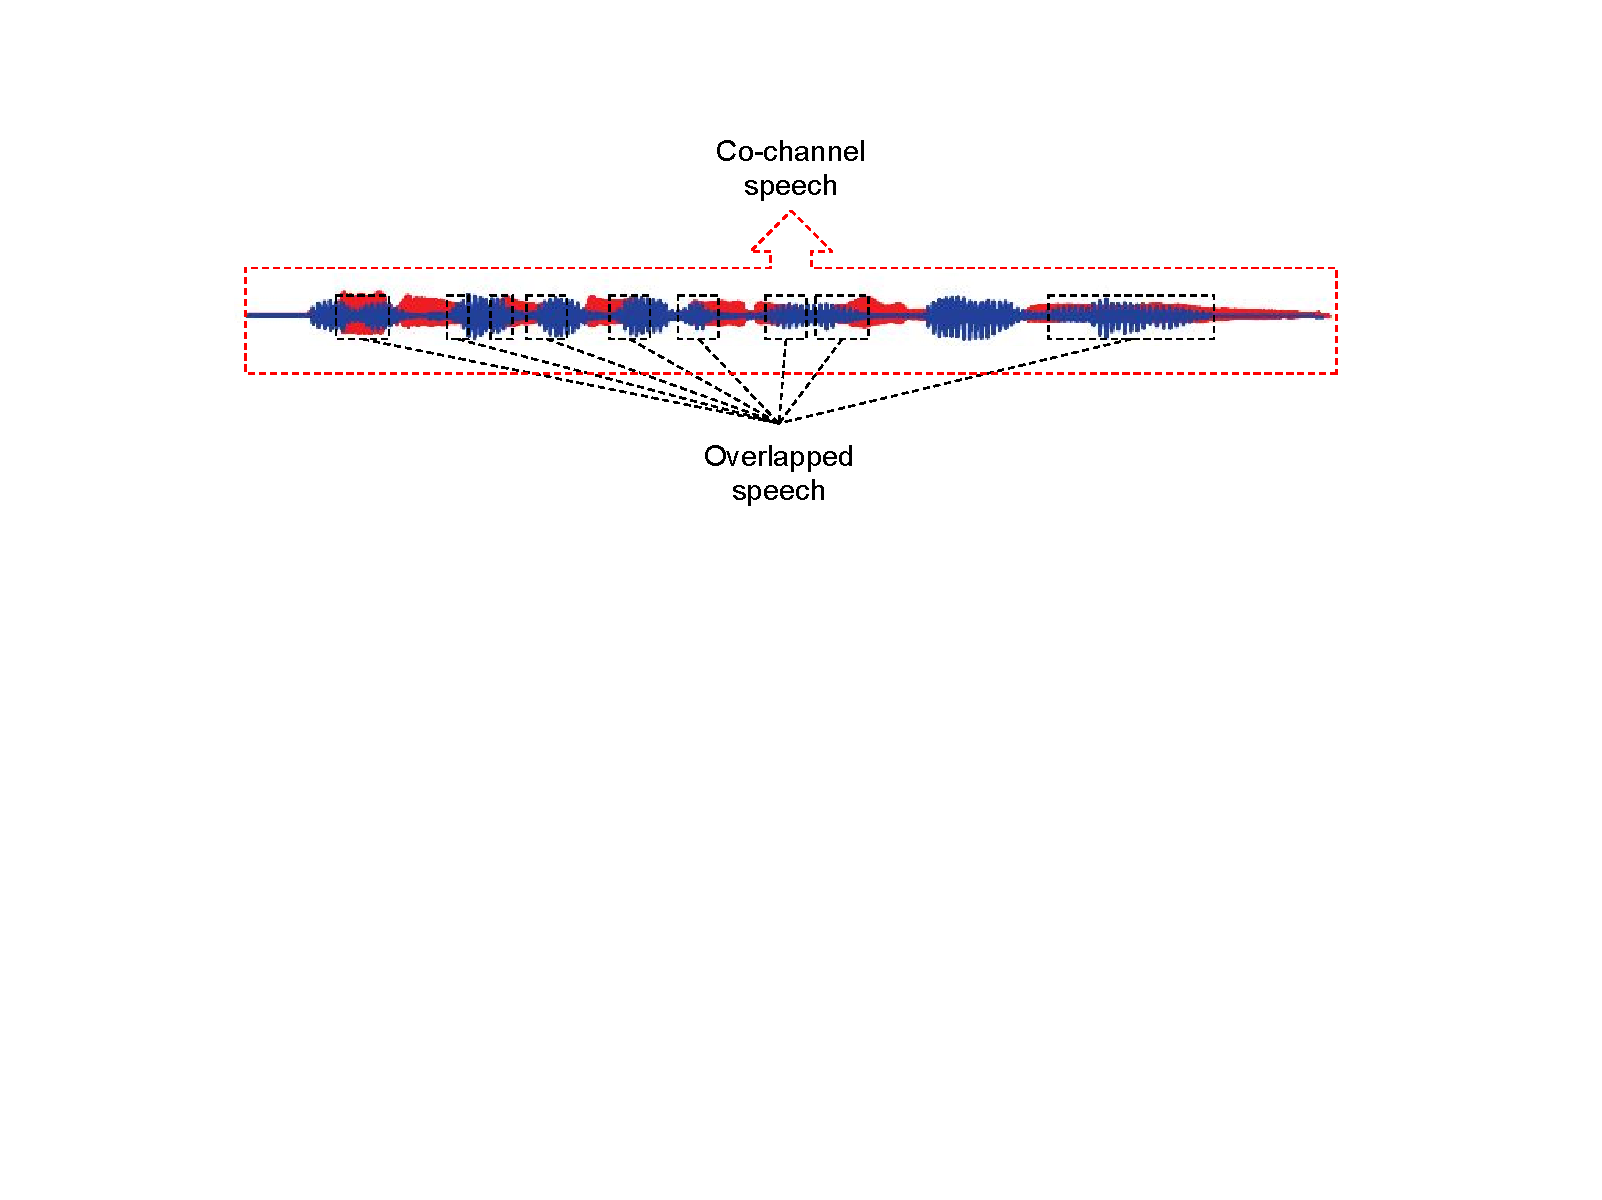
\includegraphics[height = 2in, width=0.9\textwidth]{figures/cochannel_vs_overlap-crop}
	\vspace{-3mm}
	\caption{\it \small Difference between co-channel and overlapped speech. Overlap refers to instances where more than one speaker is active. Co-channel is defined as an entire stream that contains multiple speakers. All co-channel files do not necessarily contain overlap. }
	\label{fig:cochannel_vs_overlap}
	\vspace{-3mm}
\end{figure*}


To further illustrate our problem statement, we set the following ground rules. We assume that:
\begin{itemize}
	\item There is sufficient data from multiple recording sessions for each speaker. 
	\item Recordings are co-channel and contain data from speakers other than the person of interest.
\end{itemize} 

In the standard i-vector speaker recognition framework, often a number of recordings are provided for each speaker. 
Using probabilistic linear discriminant analysis (PLDA)~\cite{prince_plda}, these i-vectors can then be reduced to a secondary subspace to compensate channel variations\footnote{Channel mismatch refers to differences in recording conditions and devices. The authors feel obligated to remind readers not to confuse channel information with co-channel speech.} across different recordings~\cite{kenny_plda,Daniel2011is}. 
Therefor, the latent variables in the PLDA subspace are calculated in a way to only represent speaker-dependent information~\cite{kenny_plda2,cumani_icassp13,burget_icassp11,yun_icassp12,matejka_icassp11}.
Now if i-vectors are to be extracted from co-channel signals, the speaker-dependent latent variables from PLDA represent a combination of all speakers in the original audio file. 
In the case of speaker recognition in co-channel speech, the task of our proposed system would be to also account for the fact that i-vectors might have been extracted from co-channel sessions. 

The aim of this study is to develop a modified version of the PLDA paradigm to make i-vectors collected from co-channel sessions usable for speaker recognition experiments and create overall robustness with respect to interfering speech. 
PLDA uses inter-session and intra-session variabilities from a development set to find a subspace in the i-vector space that best represents speaker dependencies. 
Here we investigate the possibility of performing an i-vector normalization strategy to by considering co-channel interference a form of inter-session variability.  
It is important to us that our experiments be easy to replicate and require minimal meta-data (labels, speaker and channel information, etc.). 

An investigative approach to the effects of co-channel speech in speaker recognition is presented in the next section, Sect.~\ref{sec:cochannl_in_sid}. We lay a groundwork by showing performance drop caused by adding co-channel with different signal-to-interference ratio (SIR) to enrollment and test data. 
In Sect.~\ref{sec:background}, standard PLDA and its preceding modified version, simplified PLDA, are described. We will state how channel compensation is performed through these methods~\cite{prince_plda,kenny_plda}. 
Section~\ref{sec:background} also investigates treating co-channel interference in a manner similar to how PLDA addresses channel mismatch, using a background data preparation scheme we call {\it mixed PLDA}. 
This will be followed by our proposed {\it co-channel PLDA} formulation, which is used to remove speaker interference (Sect.~\ref{sec:cch_plda}) from PLDA's speaker-dependent latent variable subspace. 
Section~\ref{sec:analysis} illustrates practical simplifications to our proposed model and analyzes its convergence behavior. 
Section~\ref{sec:exp} describes our experimental framework and presents results co-channel PLDA results. 

\section{Effect of Co-channel in Speaker Verification}
\label{sec:cochannl_in_sid}

\begin{figure*}[t!]
	\centering
	\vspace{0mm}
	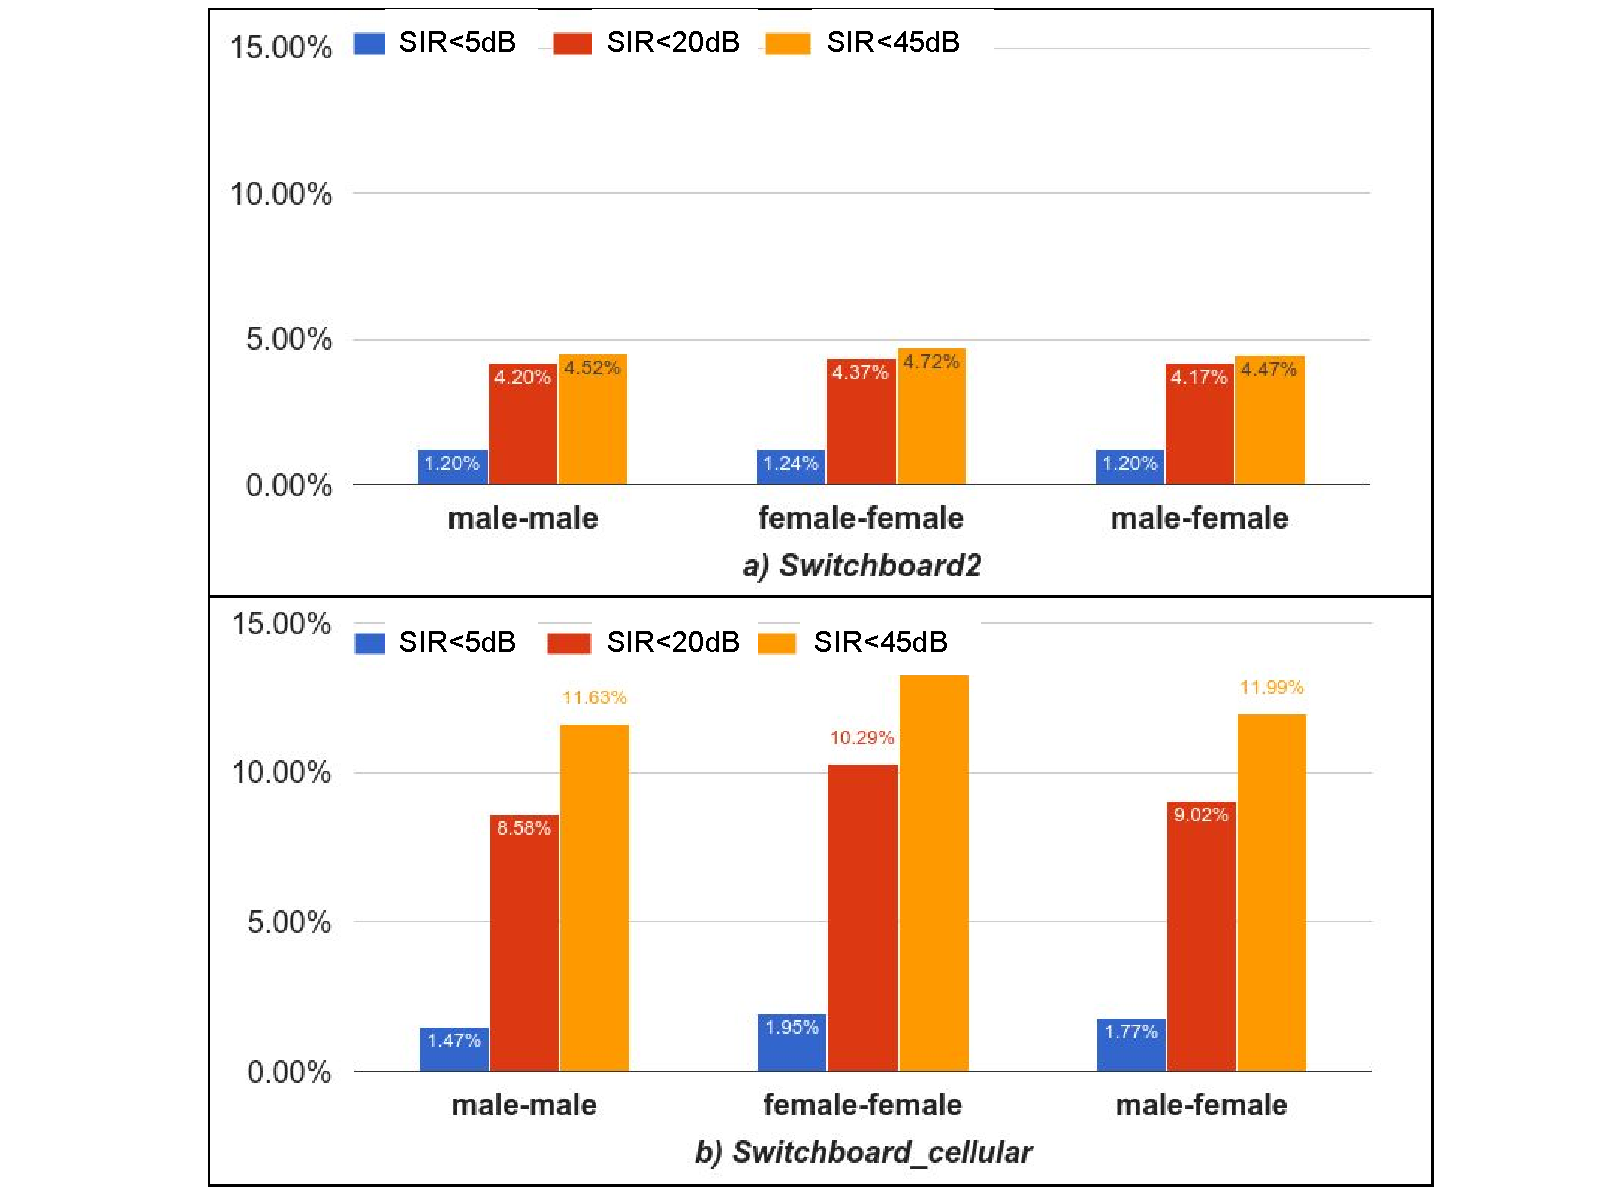
\includegraphics[height = 3.5in, width=0.8\textwidth]{figures/swb_overlap_percentage-crop}
	\vspace{-1mm}
	\caption{\it \small Percentage of overlaps to total speech in Switchboard2 and Switchboard cellular telephone conversations. Three SIR upper bounds are selected to label overlaps; 5dB, 20dB, 45dB. The higher the SIR upper bound, the stricter the overlap labels. Separate results are shown for male-male, male-female, and female-female conversations.}
	\label{fig:swb_overlap_percentage}
	\vspace{-3mm}
\end{figure*}


The first step to addressing the problem of co-channel speech compensation in speaker verification is to establish a quantitative perspective as to how much performance degradation one should expect. 
There have been a number of studies that have investigated ``co-channel speech'' and its effect on speaker verification. 
However, each provides different insight due to the somewhat nuanced definition of co-channel, as explained in the introduction. 
Many consider overlap synonymous to co-channel, which we strongly argue against in this study. 
In~\cite{yantorno_report}, co-channel speech in the form of overlaps significantly increases equal error rates for speaker verification systems based on Gaussian mixture models (GMM). 
An interesting result presented in~\cite{yantorno_report} is that a strict removal of all overlaps does not yield optimal performance, but rather keeping all ``usable speech'' leads to best performance under co-channel.  
Therefore, usable speech detection was proposed instead overlap detection to improve speaker verification performance, which has become a standard approach to addressing overlapped speech in speaker verification~\cite{Dwang_03, Dwang_03_trans}. 
In a sense, usable speech refers to speech from the foreground speaker (speaker of interest) with high signal-to-interference ratio and/or all voiced segments of the foreground speaker in which spectral harmonic patterns have not been severely disrupted~\cite{smolenski_tut}. 
Another analytic study on overlap in speaker verification was presented in~\cite{navid_pyknogram_jp}, where authors show that adding overlap to test data results in more performance degradation compared to train data. 
The authors argue that an averaging effect occurs when multiple instances of overlapped training data is provided in enrollment sessions, while test data usually has a more direct role in deriving likelihood ratios for each trial. 
An alternative to removing overlapped segments for speaker recognition has been to perform speaker separation~\cite{saeidi2010signal, mowlaee2010joint}, or in some cases simultaneous identification of both speakers in an overlapped stream~\cite{zhao2015cochannel, sadjadi_heck_icassp14}. 
We see the main theme in many of these studies, which has been to focus on overlapped speech, rather than the more general case of co-channel speech. 
Although overlap presents an undeniably difficult challenge in speaker verification, one can argue that the amount of overlap in conversational co-channel speech is far too small to pose a significant threat to speaker verification performance in large scale verification problems such as NIST speaker recognition evaluations, where in many cases sufficient data is provided. 
Later in this section, we will separately evaluate system performance under overlap-only conditions. But first, a useful analysis would be to see exactly what percentage of everyday conversational data contains overlaps. 
Readers are encouraged to visit~\cite{shriberg_01} for a detailed analysis of overlaps in conversational speech corpora. 


\begin{figure}[b!]
	\vspace{0mm}
	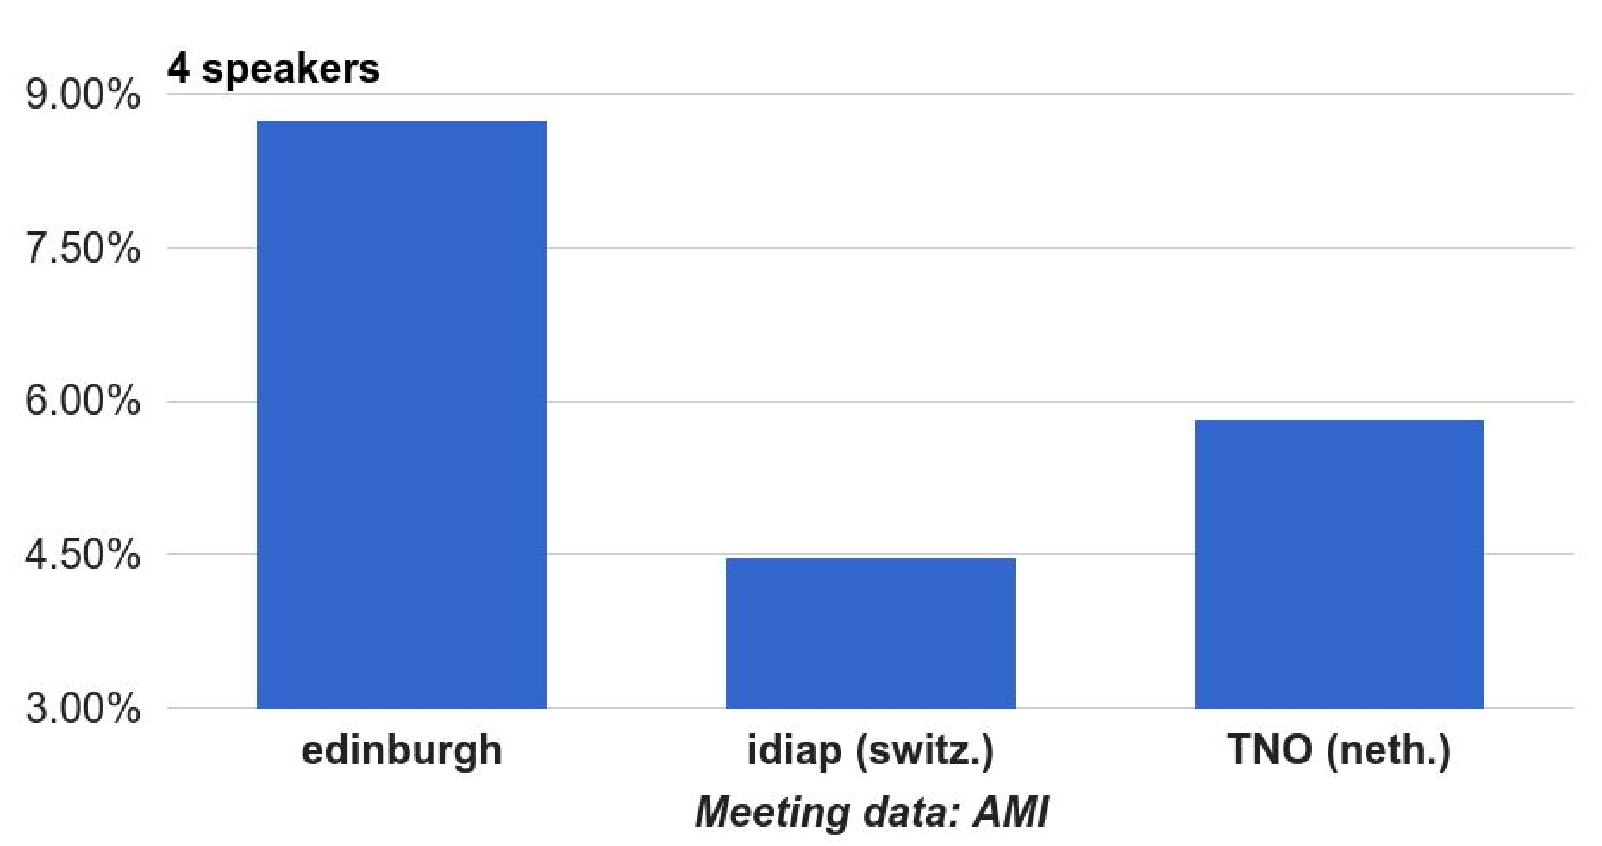
\includegraphics[height = 2.2in, width=0.5\textwidth]{figures/ami_overlap_percentage-crop}
	\vspace{-3mm}
	\caption{\it \small Percentage of overlaps to total speech in the AMI meeting corpus. All meetings used here have exactly 4 speakers. 
		The percentage of overlap is significantly higher here compared to Switchboard (compare with blue bars in Fig.~\ref{fig:swb_overlap_percentage}).}
	\label{fig:ami_overlap_percentage}
	\vspace{-3mm}
\end{figure}


Three popular corpora are investigated here: 
\begin{itemize}
\item Switchboard2: a large collection of five minute telephone conversations involving several hundred speaker from across the United States.
\item Switchboard Cellular: five-six minute telephone conversations on cellular phones.
\item AMI meeting corpus: A dataset consisting of 100 hours of meeting recordings from several locations across Europe. 
\end{itemize}

To estimate overlap in Switchboard2 and Switchboard Cellular, the separate (almost interference-free) channels provided for each speaker are first segmented into speech and silence using an energy based voice activity detection. 
Signal energies are required at each time-sample, since signal-to-interference ratio (SIR) is used to define overlap. 
Note that we use absolute SIR, since none of the speakers are favored in this scenario. 

\begin{equation}
\label{eq:abs_sir}
SIR(n) = |10log_{10}(\frac{P_1(n)}{P_2(n)})|
\end{equation}
where $P_1(n)$ is the per-sample energy of channel 1 and $P_2(n)$ corresponds to channel 2. 

The channels are mixed (per sample addition of the two signals) to create co-channel data. 
Instances at which both speakers are active are considered overlapped. 
Since the SIR value varies for different segments, overlaps are thresholded. 
Segments with SIR lower than the threshold are considered overlapped.
The amount of overlap varies with the maximum allowable SIR set by the evaluator. 
For instance, one might consider the mere presence of two speakers at the same time sufficient to label a segment as overlap, which is an indication of high SIR thresholds ($45dB$ in Fig.~\ref{fig:swb_overlap_percentage}). 
A more pragmatic view, however, is to choose an SIR small enough to preserve as much data possible for the sake of not loosing speaker recognition performance as a result of less data. 
This pragmatic view is shared in many studies under the definition of usable speech~\cite{yantorno_report}. 
Of course lower SIR values, $(0-5) dB$, have a more significant impact on speaker verification. But to provide more insight to the reader, three SIR upper bounds have been used in Fig.~\ref{fig:swb_overlap_percentage}; $5$, $20$, $45dB$. 
We argue that any overlap up to $5dB$ should have noticeable impact on speaker verification. 
An upper bound of $45dB$ is also chosen, since the percentage of overlap converges beyond $45dB$. 
We see that with a $5dB$ threshold, the percentage of overlap to total speech is below $2\%$. 
For the curios reader, we have provided overlap percentages for three groups of conversations: male-male, male-female, and female-female pairs. 
It is clear that gender does not play a role in dictating overlap percentage, at least in Switchboard.  

For a broader perspective, we also analyze the AMI meeting corpus. 
The difference between meetings and phone conversations is in the number of speakers and face-to-face interaction. 
we speculate that number of speakers increases overlap while on the other hand the fact that all speakers are present in the same room (i.e., face-to-face interaction) limits the amount of overlap. 
Another difference is that SIR is not as well defined for meetings as it is for two-party phone-calls, since multiple parties may be active at the same time. 
In Fig.~\ref{fig:ami_overlap_percentage}, we assume at least two speakers should have a relative SIR of up to $5dB$. 
Any additional speaker is evaluated with respect to the primary speaker, but with a $20dB$ threshold. 
As Fig.~\ref{fig:ami_overlap_percentage} suggests, location also plays a significant role in overlap percentage. 
The authors refrain from speculating the impact of location, since it exceed the scope of this study. 

In text-independent speaker recognition, where we are interested in long-term acoustic characteristics, 4-5\% of overlapped speech in our data has little effect on speaker recognition accuracy. The point here is not to say that overlapped speech can be neglected in speaker recognition, but to clarify that speaker recognition in its most common form is more concerned with co-channel speech in general rather than {\it overlap} as it appears in everyday English conversations. 
In the more general case of co-channel speech interference, the presence of secondary speakers has a significant impact on speaker verification. 
We roughly estimate that in a two-party phone conversation, approximately $50\%$ of the data contains the unwanted secondary speaker (compare this with $2\%$ in Fig.~\ref{fig:swb_overlap_percentage}). 


\section{Motivation}
\label{sec:background}
This section provides a brief overview of the chronological introduction and development of probabilistic linear discriminant analysis (PLDA) in speaker recognition. 
PLDA was initially proposed for face recognition in~\cite{prince_plda}. 
It was later adopted as a channel compensation step for speaker recognition using i-vectors~\cite{kenny2010bayesian}. 
A number of studies since then have presented different formulations for the factor loading paradigm most commonly known as PLDA. 
In this study, we are specifically interested in three formulations: 1) standard PLDA~\cite{kenny_plda}, 2) simplified PLDA~\cite{kenny_plda2,Daniel2011is}, and 3) the two-covariance model~\cite{brummer2010twocov}. 
The nomenclature used here is adopted from a recent study by Sizov et al.~\cite{sizov2014unifying} aimed at unifying the variations proposed for PLDA over the past decade. 


\subsection{Standard PLDA}
\label{ssec:standard_plda}
The general idea of probabilistic linear discriminant analysis is to find a subspace in a given feature space that best resembles a subset of the original space's factors. 
In the case of speaker recognition, the subset of interest contains speaker specific components. 
The search for this subspace is based on a training dataset organized in a way that emphasizes differences between speakers as well as variations of each speaker across different recordings (aka sessions). 
The data organization is comprised of $n_i$ observation i-vectors for speaker $i$ from a set of development speakers, PLDA assumes the following linear factorization for each i-vector ${\bf m}_{ij}$: 

\begin{equation}
\label{eq:std_plda}
{\bf m}_{ij} = {\bf V}{\bf y}_i+{\bf U}{\bf x}_{ij}+{\bf z}_{ij},  \hspace{30pt} j=1,...,n_i
\end{equation}

where speaker- and session-dependent latent variables, ${\bf y}_i$ and ${\bf x}_{ij}$, take a standard normal distribution, $\mathcal{N}({\bf 0},{\bf I})$. ${\bf V}$ and ${\bf U}$ are typically tall matrices representing eigenvoice and eigenchannel subspaces, respectively. Eigenvoice refers to the collection factor loadings (represented in ${\bf V}$) that construct the speaker-dependent subspace. Eigenchannel refers to the session-dependent subspace. 
In addition to the eigenchannel subspace a session-dependent and normally distributed slack variable, ${\bf z}_{ij}$, is included to express session variabilities. In (\ref{eq:std_plda}), $z_{ij}$ takes a diagonal covariance matrix, $\mathcal{N}({\bf 0},{\bf \Sigma_d})$,~\cite{kenny_plda,prince_plda}. 

PLDA predicts model parameters, $({\bf V},{\bf U},{\bf \Sigma_d})$, using the expectation-maximization (EM) algorithm~\cite{prince_plda}. 
After estimating subscpace components using background development data, trial i-vectors are then reduced to the same speaker-dependent subspace (indirectly) using PLDA and scored through a hypothesis testing procedure (see~\cite{prince_plda} for details). 
The hypothesis testing stage estimates the likelihood ratio of whether two trial i-vectors (train and test) belong to the same speaker, or if they belong to two different speakers. 

\subsection{Simplified PLDA}
\label{ssec:simplified_plda}
The second formulation reduces the complexity of (\ref{eq:std_plda}) using the fact that session-dependent latent (${\bf x}_{ij}$ in (\ref{eq:std_plda})) variables are not directly used in the scoring process. 
Therefore, as long as models are able to effectively estimate the eigenvoice subspace, channel related dimensionality (essentially all non-speaker dimensionality) is redundant. 
With this in mind, the second term in (\ref{eq:std_plda}) is removed in simplified PLDA and all channel information is captured in the slack variable. 
The slack variable in this case is assumed to have a full covariance matrix.

\begin{equation}
\label{eq:simple_plda}
{\bf m}_{ij} = {\bf V}{\bf y}_i+{\bf z}^f_{ij},  \hspace{30pt} j=1,...,n_i
\end{equation}

The use of a full covariance matrix in the slack variable of simplified PLDA can be interpreted as combining the diagonal slack covariance in (\ref{eq:std_plda}) with the eigenchannel subspace projections ${\bf UU}^T$~\cite{sizov2014unifying}.


\subsection{PLDA as an extension to LDA}
\label{sec:twocov}
The last interpretation used in this study is a probabilistic extension to linear discriminant analysis (LDA), also called the two-covariance model~\cite{sizov2014unifying}, which describes the i-vector space in terms of between- and within-speaker covariances. 
LDA models a feature space as a mixture of Gaussians, in which each mixture has the same covariance of ${\bf \Phi_w}$. 
Gaussian mixtures represent within class (i.e., speaker) variability, therefore ${\bf \Phi_w}$ is referred to as the within-class covariance matrix. 
What LDA fails to provide is a continuous (or in this context, stochastic) representation of each mixture's centroid. 
Therefore, centroids are considered deterministic in LDA. 
LDA is commonly used to find the optimal discriminating subspace of a given set of training speakers, relative to there within-speaker variation~\cite{ioffePLDA2006}. 
The problem, however, is that the aforementioned subspace is only optimal for the given training speakers. 
If a new speaker is introduced, the resulting projection of LDA is not necessarily reliable.
PLDA provides a stochastic representation of class centroids using a between-class covariance matrix, ${\bf \Phi_b}$~\cite{ioffePLDA2006}. 
The stochastic centroid space assumes a continuous centroid subspace, which acknowledges the possibility of unseen speakers. 
PLDA can therefore be defined as a combination of two distributions; 
\begin{enumerate}
	\item the distribution of i-vectors in each class representing a certain speaker, which is a Gaussian with mean $s$, mean of a speaker's i-vectors, and covariance ${\bf \Phi_w}$:
	\begin{equation}
		\label{eq:within_spk_dist}
		{\bf m} \sim \mathcal{N} ({\bf s},{\bf \Phi_w}),
	\end{equation}
\item class centroid distribution, also assumed Gaussian:
	\begin{equation}
		\label{eq:between_spk_dist}
		{\bf s} \sim \mathcal{N} ({\bf s_g},{\bf \Phi_b}),
	\end{equation}
	where ${\bf s_g}$ is the global mean of all class centroids and ${\bf \Phi_b}$ is the between-speaker covariance matrix. 
\end{enumerate}

Defining channel variability as a function of speaker variation helps PLDA model unseen speakers (i.e., speakers that are not present in the development set), which LDA is incapable of doing~\cite{ioffePLDA2006}. 
The interpretation in this section, provides a perspective which we will use in our proposed method (Sect.~\ref{sec:method}) to include co-channel interference as a contributor to within-class variability. 
Equations (\ref{eq:within_spk_dist}) and (\ref{eq:between_spk_dist}) can be derived from (\ref{eq:simple_plda})~\cite{sizov2014unifying} or vice versa~\cite{ioffePLDA2006}. 
 

\subsection{Baseline: mixed PLDA}
\label{ssec:plda_data_prep}
The search for eigenvoice and eigenchannel subspaces involves a careful selection of development data. 
The idea in data preparation for PLDA is to provide sufficient channel diversity for each speaker to model within-speaker variations, while maintaining high speaker counts to be able to model between-speaker variability. 
Channel and speaker diversities introduced in the development data are directly translated into within- and between-speaker covariances, respectively. Said covariances are used to estimated PLDA parameters, (\ref{eq:std_plda}) and (\ref{eq:simple_plda})~\cite{sizov2014unifying}. 
Such a data driven perspective towards channel compensation using PLDA has inspired a number of studies to tackle other types of variability through the same data selection procedure. 
Thereby, instead of channel diversity, one could generate a development set with age diversity~\cite{kelly2014thesis} or language diversity~\cite{misra2014languagemismatch} (in the case of multi-lingual speakers). 
This leads to our first approach, which is to establish the amount of achievable performance gain in co-channel speaker recognition when background PLDA data contains co-channel speech samples. 
In this approach, recordings for each speaker consists of multiple co-channel samples. 
Note that it is important to maintain diversity in secondary (aka interfering) speakers, otherwise the PLDA model will train to both primary and secondary speakers in co-channel sessions. 
Figure~\ref{fig:mixedPLDA_diagram} is a diagram of how the PLDA data is arranged in this baseline approach, which we call ``mixed PLDA''. 
Mixed PLDA implicitly compensates speaker interference in the background development data using co-channel mixtures. 


\begin{figure}[t!]
	\centering
	\vspace{0mm}
	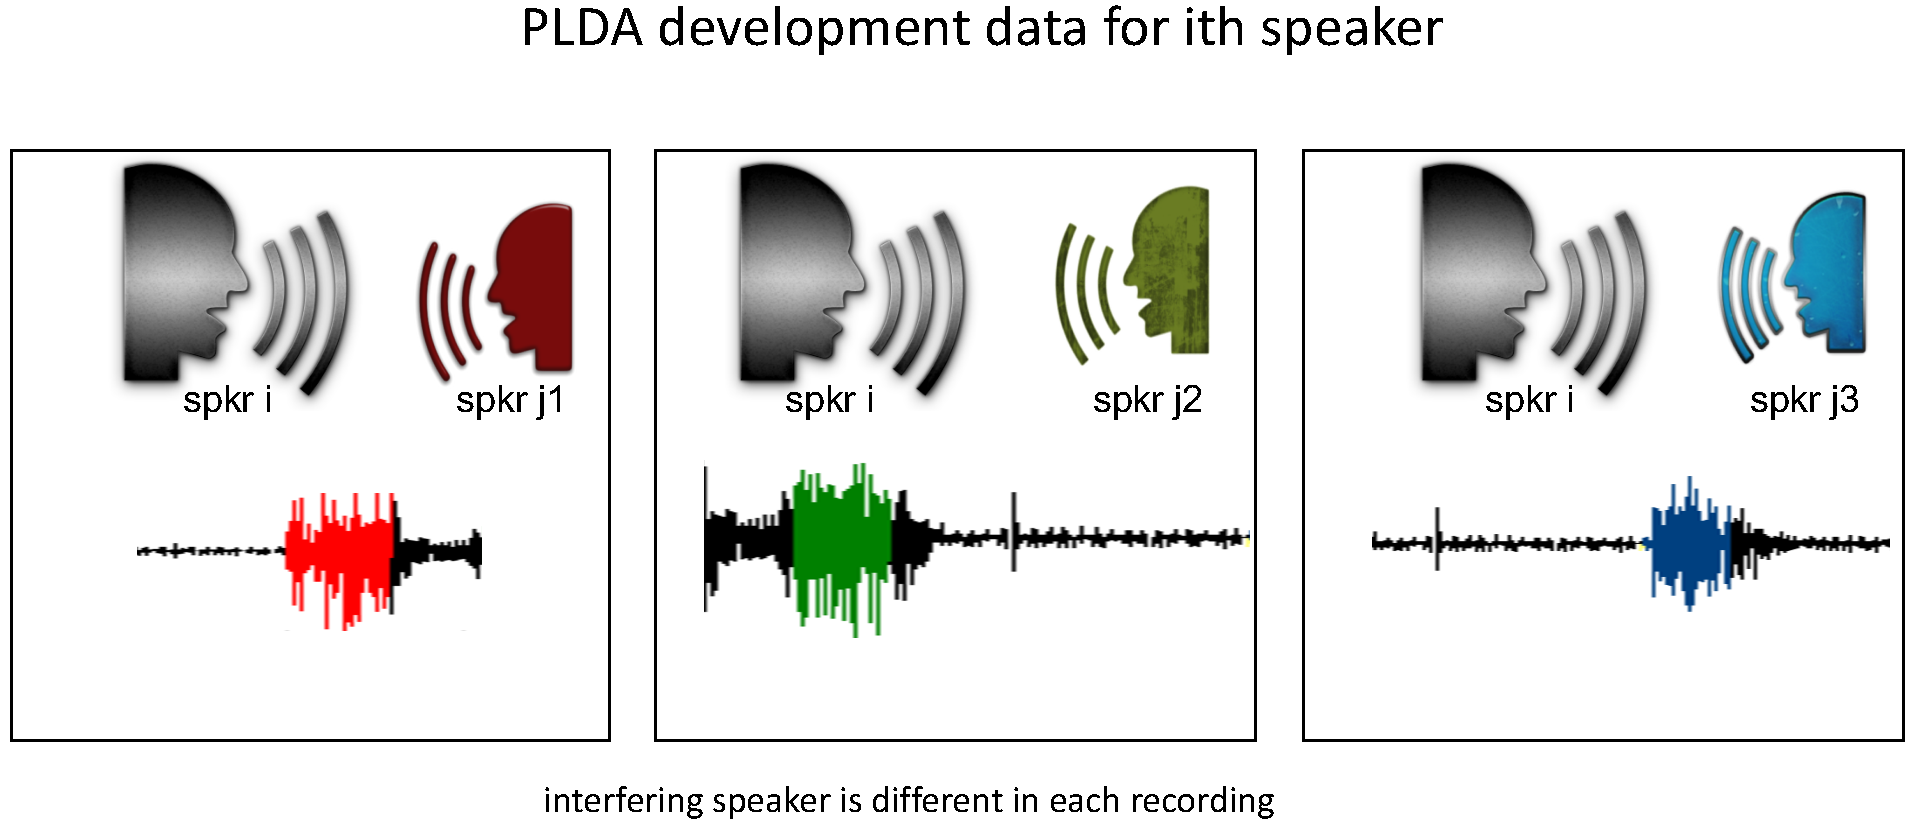
\includegraphics[width=0.5\textwidth, height=1.8in]{figures/mixedPLDA_slide-crop}
  	\vspace{-5mm}
	\caption{\it \small Creating development data for co-channel aware PLDA. the mixed PLDA approach uses co-channel data for each speaker in the background model. Recordings for the $i^{th}$ speaker consists of co-channel sessions with different speakers.}
	\label{fig:mixedPLDA_diagram}
	\vspace{-3mm}
\end{figure}

Mixed PLDA describes the use of co-channel background data in simplified and standard PDLA formulations of equations (\ref{eq:simple_plda}) and (\ref{eq:std_plda}). 
This will be used as a baseline to provide fair comparison with our proposed PLDA formulation described in the next section, since (\ref{eq:std_plda}) and (\ref{eq:simple_plda}) do not claim robustness with respect to co-channel data in their original forms. 


\section{Proposed method: Co-channel Aware PLDA}
\label{sec:cch_plda}
This section describes our proposed approach, which is a modification to the PLDA formulation (Sect.~\ref{sec:background}) that allows modeling speaker interference. 
Previously, in~\cite{shokouhi2015probabilistic}, we proposed a modified PLDA formulation to remove secondary speaker interference from the latent variable subspace. 
This study proposes a different method based on the two-covariance interpretation (described in Sect.~\ref{sec:twocov}). 
The proposed method in this study, which we call {\it co-channel aware PLDA} (caPLDA), integrates the between-speaker covariance matrix into the within-class covariance to further emphasize the uncertainty caused by interfering speakers. 
Part of the reason for our departure from the co-channel PLDA formulation proposed in~\cite{shokouhi2015probabilistic} was our inability to justify certain behavior in the model~\cite{navid_phd_thesis}. 
The current formulation (i.e., caPLDA), however, uses a sounder approach to combine co-channel interference with session variability. 

caPLDA adopts the two-covariance interpretation of PLDA briefly described in (\ref{eq:within_spk_dist}) and (\ref{eq:between_spk_dist}). 
The i-vectors of a given class can be modeled as a normally distributed vector with a mean pertaining to the class to which it belongs and a covariance matrix representing within class variability, (\ref{eq:within_spk_dist}). 
Typically, within-class variability is meant to model channel variation across sessions. 
In the case of co-channel speech, in addition to channel variability, one must consider the variability caused by interfering speakers. 
In Sect.~\ref{ssec:plda_data_prep}, we attempted to capture speaker interference in the same manner channel variation is captured by PLDA. 
Although some improvement is observed, we expect that the original PLDA formulation, (\ref{simple_plda}), is not capable of fully capturing speaker interference; partly due to the similarity between speaker-dependent latent variables and the cross session variations that exist in co-channel interference. 
We propose that in order to further improve performance, information can be shared between the speaker-dependent covariance matrix (between-speaker covariance) and the within-class covariance computed in the mixedPLDA method from Sect.~\ref{ssec:plda_data_prep}. 
For an i-vector with speaker $A$ as the foreground speaker and some speaker $X$ as secondary speaker, PLDA assumes this i-vector is generated from a normal distribution $\mathcal{N} {m_A,\Phi}$. 
While (\ref{sec:twocov}), assumes $\Phi$ is a unique within-class covariance matrix for all speakers in the i-vector space (i.e., $\Phi_w$), we argue that an additional component is required to model within speaker variations in the case of co-channel i-vectors. 
The additional component contributing to within-class covariance is of the same nature of the between-class covariance. 
Therefore, one can assume that $\Phi$ is a function of both $\Phi_w$ and $\Phi_b$ (as defined in Sect.~\ref{sec:twocov}), $ \mathcal{F} (\Phi_w,\Phi_b)$. 
Our suggested structure for $ \mathcal{F} (.,.)$ is a linear combination of the two covariance matrices: 

\begin{equation}
\Phi = \mathcal{F} (\Phi_w,\Phi_b) = 
\Phi_w + \alpha\Phi_b
\end{equation}
where $\alpha$ is a function of the signal-to-interference ratio between the foreground and background speaker. 
For clean (non co-channel) i-vectors, $\alpha$ should be $0$, while $\alpha$ increases as SIR drops. 
Note that the typical scale of the $\Phi_b$ is much large than $\Phi_w$~\cite{glembek2014wccLDA}, therefore the range of $\alpha \in (0,\alpha_{max})$ is chosen such that $\alpha_{max} << 1$.

\section{Experiments}
\label{sec:exp}

\subsection{Co-channel Interference in Trials}

In this section, a series of speaker verification experiments are conducted on Switchboard2 to demonstrate the effect of using co-channel speech in enrollment and test data. 
We do not introduce these experiments as ``baseline'', since adding co-channel interference to trials and expecting PLDA to perform well is an unfair assessment. 
The purpose of this section is to show the increase in equal error rates as a result of co-channel speech. 
We also further emphasize the point made in Sect.~\ref{sec:cochannl_in_sid} by identifying the impact of overlap from co-channel interference on the EER. 

For these experiments, single-speaker data is used to estimate PLDA parameters (not co-channel data). 
Trials are evaluated at different levels of co-channel interference (i.e., SIR level). 
In each scenario, trial recordings are summed with their counterpart channel from the phone conversation to create co-channel data, as if speakers are speaking on a single channel (shown in Fig.~\ref{fig:mix_swb}). 
Speaker labels for trial recordings are generated based on the foreground speaker. 
In this context, foreground speaker refers to the speaker of interest. 
For example, in a $5dB$ co-channel session generated from Switchboard2 containing speakers {\bf X} and {\bf Y}, if {\bf X} were the foreground speaker, the average energy of {\bf X} would be $5dB$ higher than the average energy of {\bf Y}. 
Therefore, $SIR_{trial}$ is defined slightly differently from here on after, compared to the per-sample absolute $SIR(n)$ in (\ref{eq:abs_sir}). 
\begin{equation} 
SIR_{trial} = 10log_{10}\Big(\frac{\frac{1}{T}\sum_t E_X(t)}{\frac{1}{T}\sum_t E_Y(t)}\Big), \hspace{30pt} t=1,...,T
\end{equation}
where $E_X(t)$ and $E_Y(t)$ are signal energies at frame $t$. 
Five SIR levels are chosen throughout experiments; $100dB$ (i.e., clean sessions), $20dB$, $10dB$, $5dB$, and $0dB$. 
In $0dB$ the average energy of the foreground and background data is equal. 
To avoid mismatch, the clean condition is also generated through the same procedure with an SIR of $100dB$ favoring the foreground speaker. 

A gender-independent universal background model (UBM) is created using 8kHz single-speaker NIST SRE data from 2004, 2005, and 2006 challenges~\cite{NIST04,NIST05,NIST06}. 
The UBM consists of $2048$ Gaussian mixtures representing a 39 dimensional feature space (13 dimensional MFCC plus $\Delta$ and $\Delta\Delta$). 
The same data from SRE 2004-6 is used to estimate a total variability (TV) matrix, which extracts $400$ dimensional i-vectors~\cite{Dehak_ivector}. 
The data used here to estimate PLDA parameters are single-speaker recordings from NIST SRE 2008~\cite{NIST08}. 
PLDA training data consists of approximately $11k$ single-speaker utterances from over $1300$ speakers. 
Trial data is developed from 2500 Switchboard2 recording sessions containing approximately $800$ speakers. 
Prior to feature extraction, trials are processed using comboSAD, an unsupervised speech activity detection~\cite{sadjadi2013unsupervised}, which has previously shown to provide stable performance improvement in such speaker recognition tasks~\cite{hasan2013crss}. 

\begin{figure}[t!]
	\vspace{-1mm}
	\hspace{3mm}
	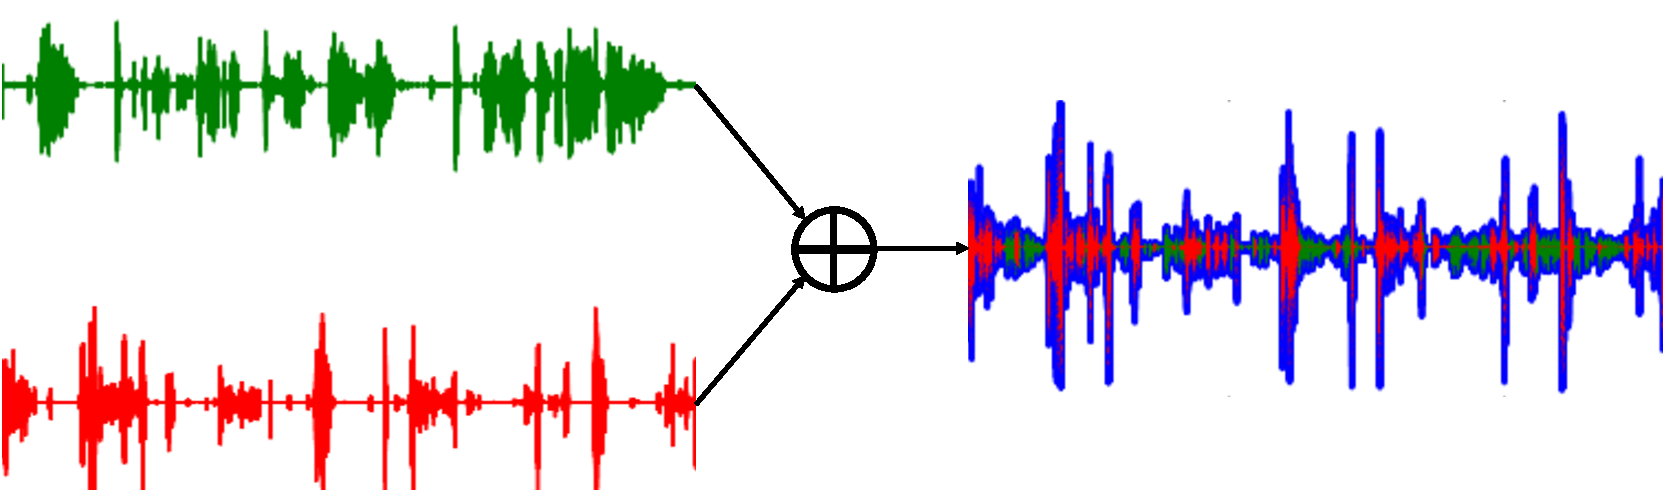
\includegraphics[height = 1.0in, width=0.45\textwidth]{figures/swb_cch_demo-crop}
	\vspace{-1mm}
	\caption{\it \small Mixing two channels of a Switchboard phonecall. The example here mixes the signals with 0dB SIR. Blue shows the resulting co-channel signal. Red and green each show one of the single-speaker signals.}
	\label{fig:mix_swb}
	\vspace{-1mm}
\end{figure}

Figure~\ref{fig:cch_in_sid} shows speaker verification performance for the five SIR cases. 
As shown, EER for the clean condition is significantly lower than all the other SIR levels, even $20dB$. 
The sudden jump in EER shows the significance of co-channel interference. 

\begin{figure}[h!]
	\vspace{-1mm}
	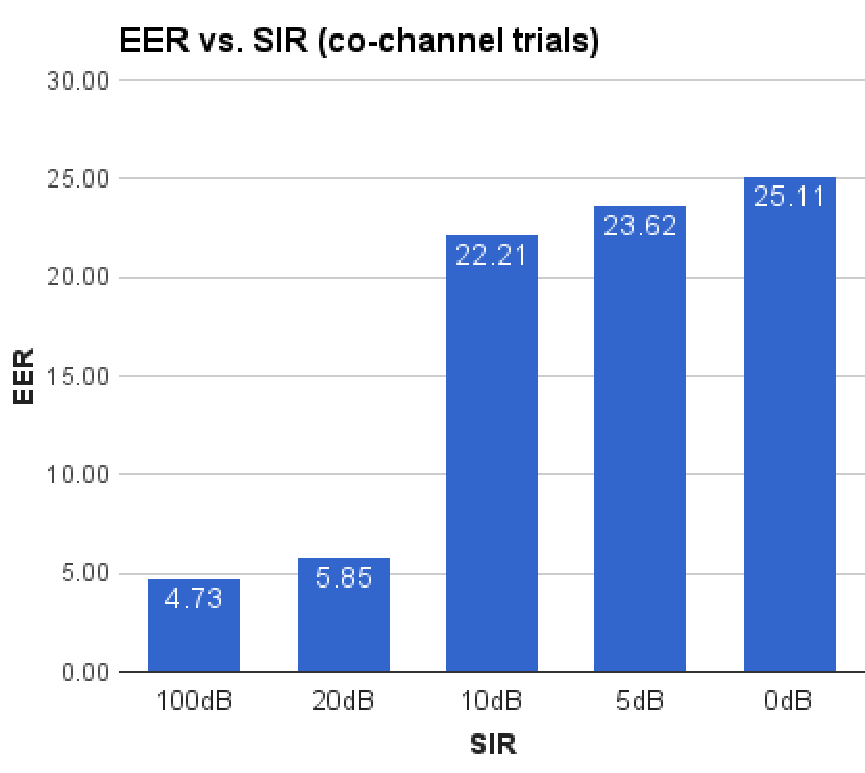
\includegraphics[height = 2.5in, width=0.48\textwidth]{figures/eer_vs_sir_swb2_baseline}
	\vspace{-2mm}
	\caption{\it \small Speaker verification performance with co-channel speech in switchboard trials. The i-vector/PLDA system uses a typical system configuration and is fully trained on single-speaker data. The purpose of this chart is to show the rapid increase in equal error rate (EER) as co-channel data is added to the trials. 100dB SIR represents clean (single-speaker) trials.}
	\label{fig:cch_in_sid}
	\vspace{-1mm}
\end{figure}


A second experiment is conducted to separate performance drop caused by overlap. To show this, all speech from the secondary speaker is dropped from the recordings, except for segments that overlap with the foreground speaker. 
This is accomplished by using voice activity detection (VAD) labels from the 100dB trials, while using $0dB$ audio data for the trials. 
Figure~\ref{fig:ovl_in_sid}, compares speaker verification under overlap with 0dB co-channel speech. 

\begin{figure}[h!]
	\vspace{-1mm}
	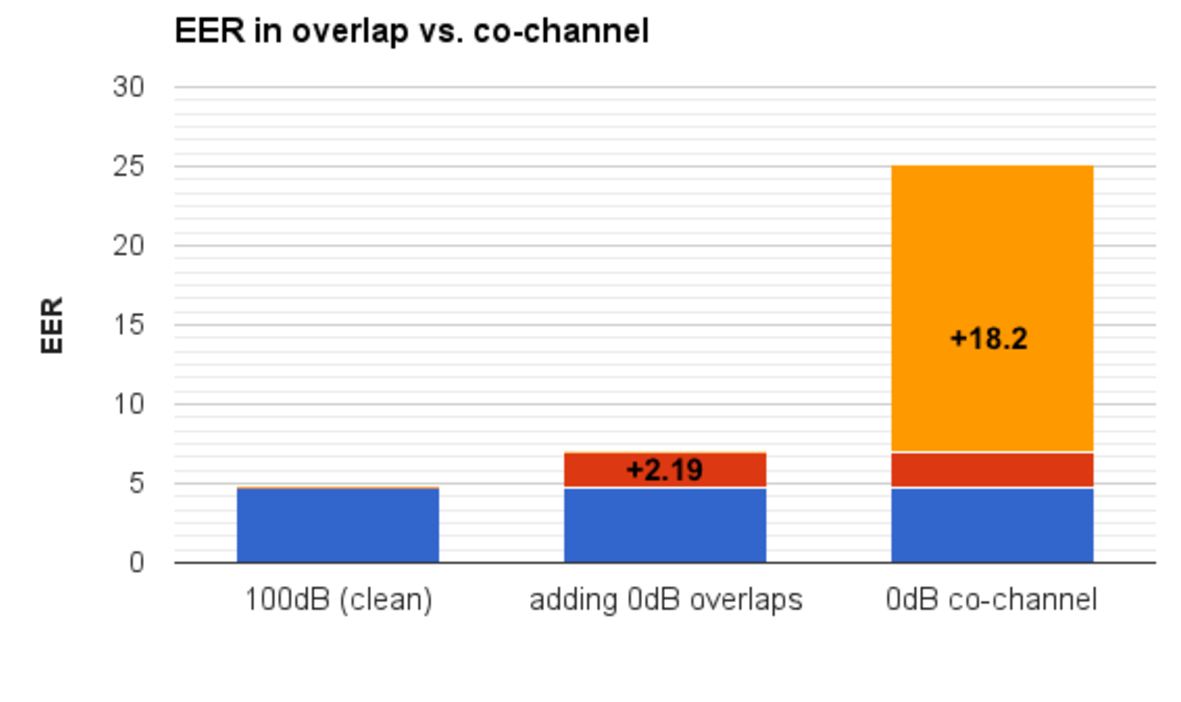
\includegraphics[height = 2.5in, width=0.5\textwidth]{figures/overlap_vs_cochannel_sid-crop}
	\vspace{-8mm}
	\caption{\it \small Comparing the effect of overlap in speaker verification with the more general case of co-channel. This study differentiates overlap from co-channel speech by considering overlaps to be segments during which both speakers are active. Co-channel refers to the more general case of two speakers in an audio stream, not necessarily overlapped (see Fig.~\ref{fig:cochannel_vs_overlap}). The chart shows that overlap plays a small part in the rise of EER compared to co-channel interference.}
	\label{fig:ovl_in_sid}
	\vspace{-1mm}
\end{figure}

\subsection{Co-channel Interference in Trials with mixedPLDA} 
\label{ssec:mixedplda_exp}


\section{Conclusion}
The conclusion goes here.





\ifCLASSOPTIONcaptionsoff
  \newpage
\fi

\bibliographystyle{IEEEtran}
\bibliography{IEEEtrans_refs}
\end{document}


